\chapter{Alimentation d’un microprocesseur}

On souhaite alimenter un microprocesseur STM32H4 à l'aide d'une batterie. Le cahier des charges est le suivant :

\begin{itemize}
\item Batterie LiPo 2S $V_{in} = 7.4\ V$
\item Tension d’alimentation du microprocesseur : $V_{out}=3.3\ V$
\item Ondulation de tension max en entrée du microprocesseur : $\Delta V_S = 50\ mV$
\item Courant nominal de sortie : $I_S = 200\ mA$
\item Ondulation de courant : 30\%
\end{itemize}

Pour cela, on souhaite utiliser le composant suivant : \textbf{LT1959} dont un extrait de la documentation est en annexe. On supposera dans cet exercice que les \underline{\textbf{composants sont}} \underline{\textbf{parfaits}}, et que le Buck fonctionne en régime de \underline{\textbf{conduction continue}}.

\begin{enumerate}

\item \textbf{Étude du Buck}

\begin{enumerate}

\item Tracer le circuit permettant d'utiliser ce composant en fonctionnement Buck (la valeur des composants passifs n'est pas demandée). Pour la broche 6 $\overline{SHDN}$, on supposera que le Buck est toujours en fonctionnement.

\item On suppose que le processeur absorbe un courant $I_s$ constant égal au courant nominal et que la tension de sortie est constante (on néglige l'ondulation de la tension de sortie). Tracer l'allure de la tension $V_{SW}$ en sortie du composant \textbf{LT1959}, $I_{SW}$ le courant de sortie du composant, la tension $V_{ce}$ aux bornes du transistor $Q_1$ et le courant $I_{L}$ dans l'inductance de sortie. En déduire la relation entre la tension d'entrée $V_{in}$, $V_{out}$ et le rapport cyclique $\alpha$ du hacheur.

\item Si la tension de sortie est bien régulée, quelle sera la valeur du rapport cyclique $\alpha_n$ imposé par le \textbf{LT1959} ?

\item Justifier que ce composant est adapté au cahier des charges. Peut-on utiliser une batterie LiPo 1S ($3.7 V$) à la place de la LiPo 2S ?

\item A partir de la documentation, quelle est la fréquence de découpage du hacheur ?

\item Calculer l'ondulation de courant $\Delta I_{L}$ dans l'inductance de sortie, en fonction de l'inductance $L_1$ placée. En déduire la valeur de l'inductance afin de respecter le cahier des charges.

\item Tracer la tension de sortie en tenant compte de l'ondulation de tension. Calculer la valeur du condensateur de sortie $C_1$ à choisir afin de respecter le cahier des charges.

\item Que se passe-t-il si le microprocesseur consomme peu de courant (mode veille par exemple) ?

\end{enumerate}

\item \textbf{Etude de la commande}

Dans cette partie, on s'intéresse à la commande du Buck. Pour cela, on utilise le schéma simplifié suivant :

\begin{figure}[h]
\centering
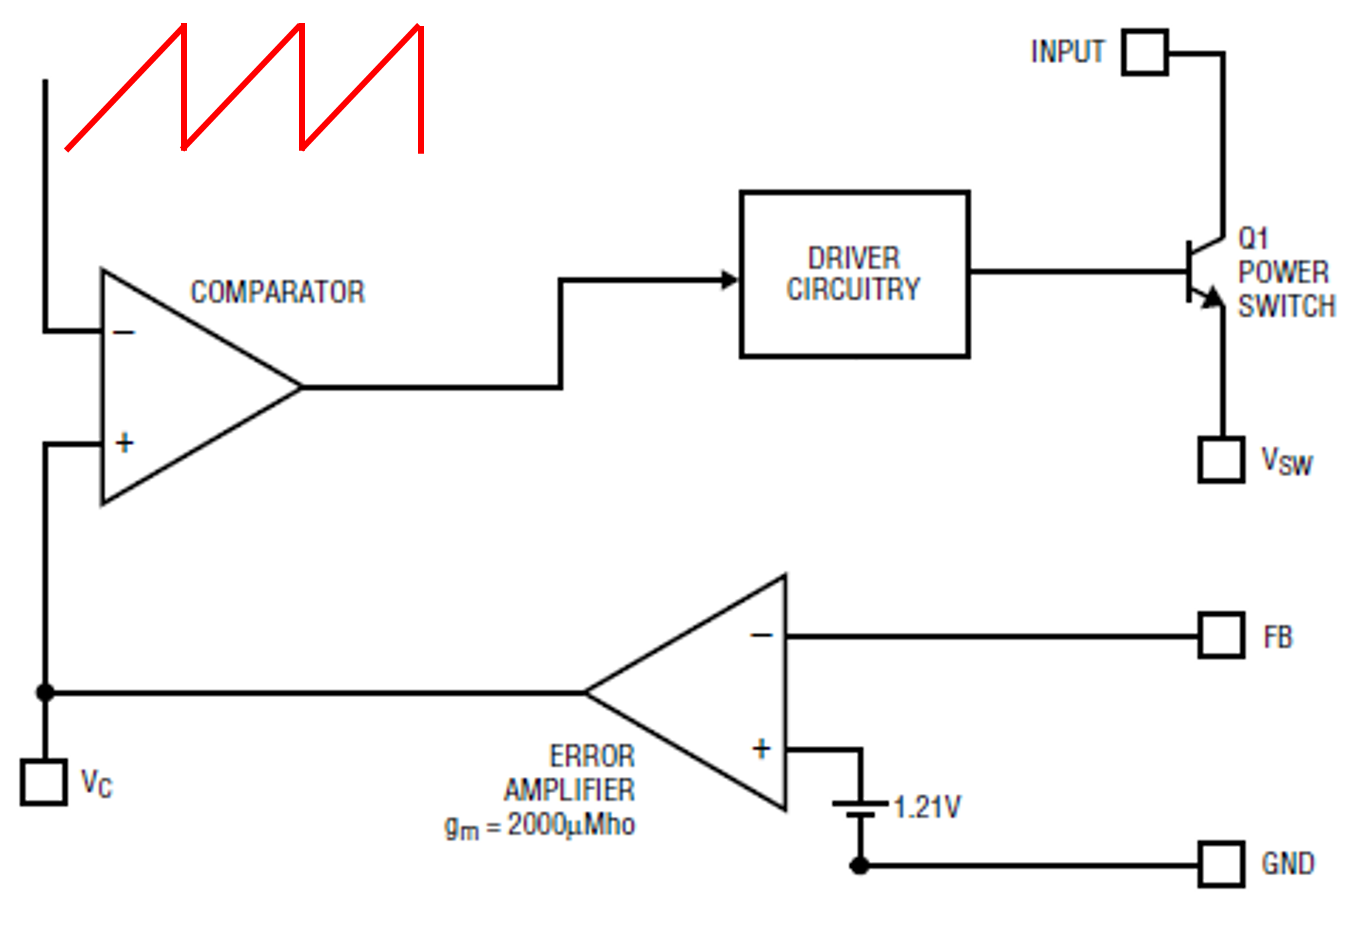
\includegraphics[width=0.8\linewidth]{TD_Buck/fig/Buck_regul.png}
\caption{Simplified internal control}
\end{figure}

Le signal en dent de scie évolue entre 0 et 2 V, avec une fréquence égale à la fréquence de découpage du hacheur. 

\begin{enumerate}

\item Choisir les valeurs des résistances à connecter sur la broche \textit{FB} afin d'avoir la tension de sortie demandée. On utilisera pour cela les valeurs de résistances de la série E12.

(Valeurs de la série E12 : 100, 120, 150, 180, 220, 270, 330, 390, 470, 560, 680, 820).

\item Pour une tension $V^+=0.5 V$ à l'entrée du comparateur, tracer le signal en sortie du comparateur. En déduire l'expression qui lie la tension $V^+$ du comparateur et la valeur du rapport cyclique $\alpha$ du hacheur.

On modélise le convertisseur asservi avec le schéma bloc suivant :

\begin{figure}[H]
\centering
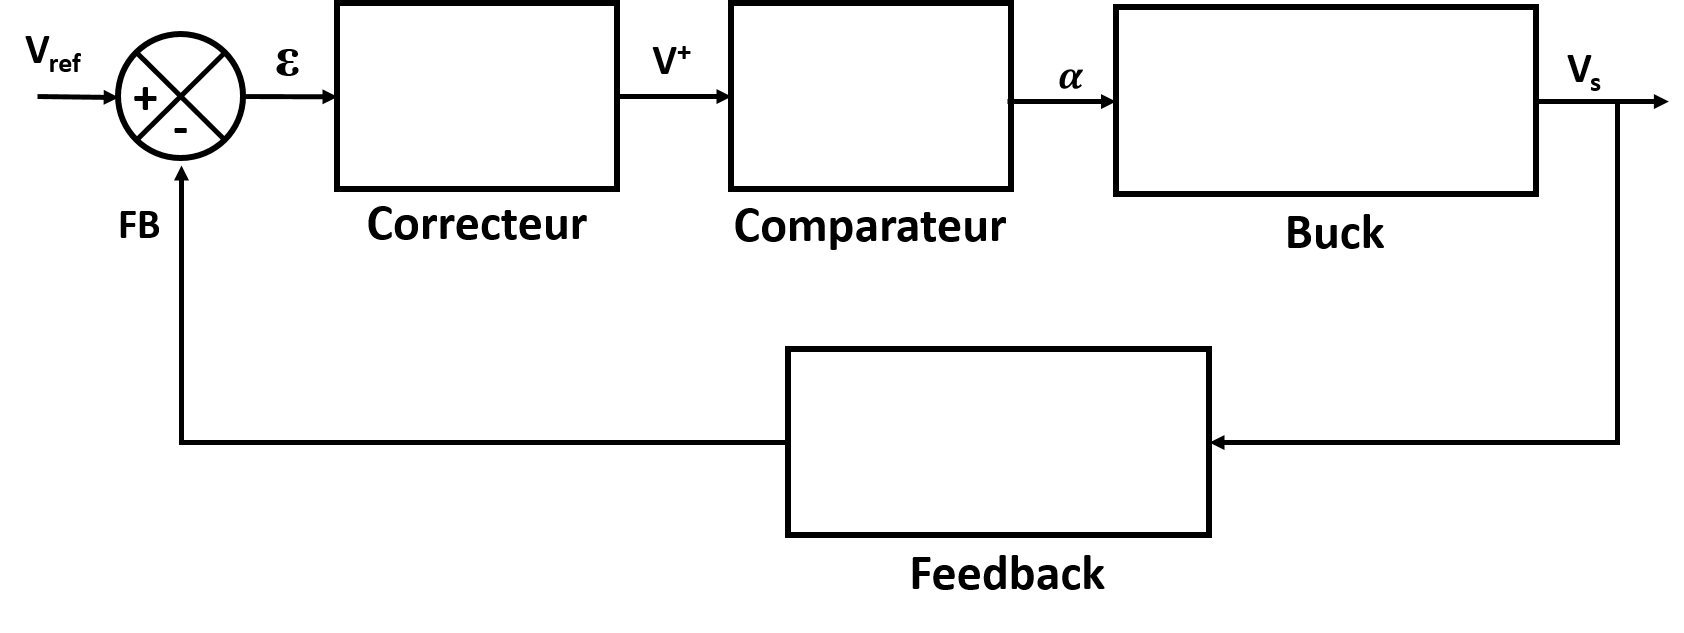
\includegraphics[width=0.8\linewidth]{TD_Buck/fig/Buck_regul_1.png}
\caption{Global bloc diagramm}
\end{figure}

\item Compléter le bloc ``\textit{Comparateur}''. A l'aide de la partie 1, compléter le bloc ``\textit{Feedback}''

Le bloc ``\textit{Buck}'' est modélisé par un gain statique $K$ correspondant à $\dfrac{V_{s\ moy}}{\alpha}$ et une fonction de transfert correspondant au filtre de sortie de Buck. La résistance $R_m$ symbolise l'impédance d'entrée du microcontrôleur.

\begin{figure}[h]
\centering
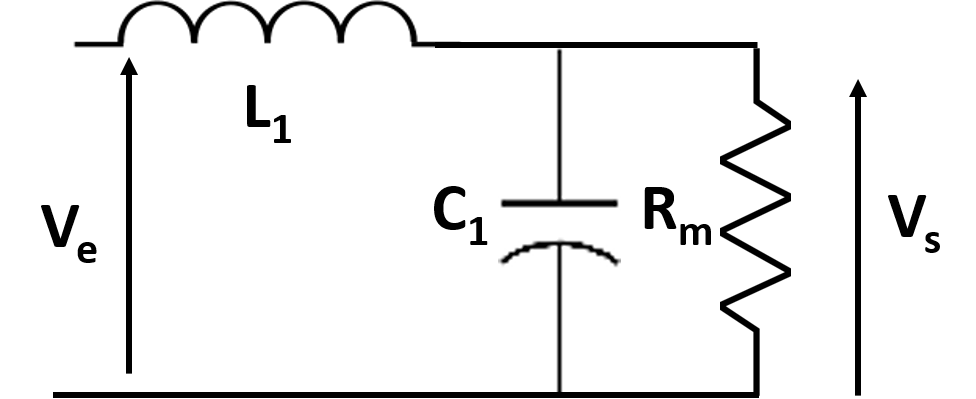
\includegraphics[width=0.55\linewidth]{TD_Buck/fig/Buck_filtre.png}
\caption{Equivalent schematic of the Buck}
\end{figure}

\item Rappeler les valeurs de $L$ et $C$ déterminées à la partie. Déterminer la valeur de $R_m$ lorsque le microcontrôleur absorbe le courant nominal.

\item Déterminer la fonction de transfert correspondant au bloc ``\textit{Buck}''.

\item On place sur la broche $V_c$ un circuit $RC$ série. On suppose que le courant en entrée du comparateur est nul (haute impédance d'entrée). Le bloc ``\textit{Correcteur}'' est donc un proportionnel intégral de la forme $C(p) = K_p(1+\dfrac{1}{T_i.p})$. Déterminer les valeurs de $K_p$ et $T_i$ en fonction de $R$, $C$ et $g_m$.

\item Calculer $R$ afin que le rapport cyclique au démarrage soit environ égal à $\dfrac{\alpha_n}{2}$ et $C$ pour avoir une constante de temps du correcteur 10 fois supérieure à la constante de temps du système non corrigé.

\item En régime établi, déterminer le courant de sortie de l'ampli d'erreur et les tensions aux bornes de $R$, $C$ et $V_c$. En déduire le rapport cyclique et comparer au résultat du 1.3.


\end{enumerate}

\end{enumerate}

\newpage
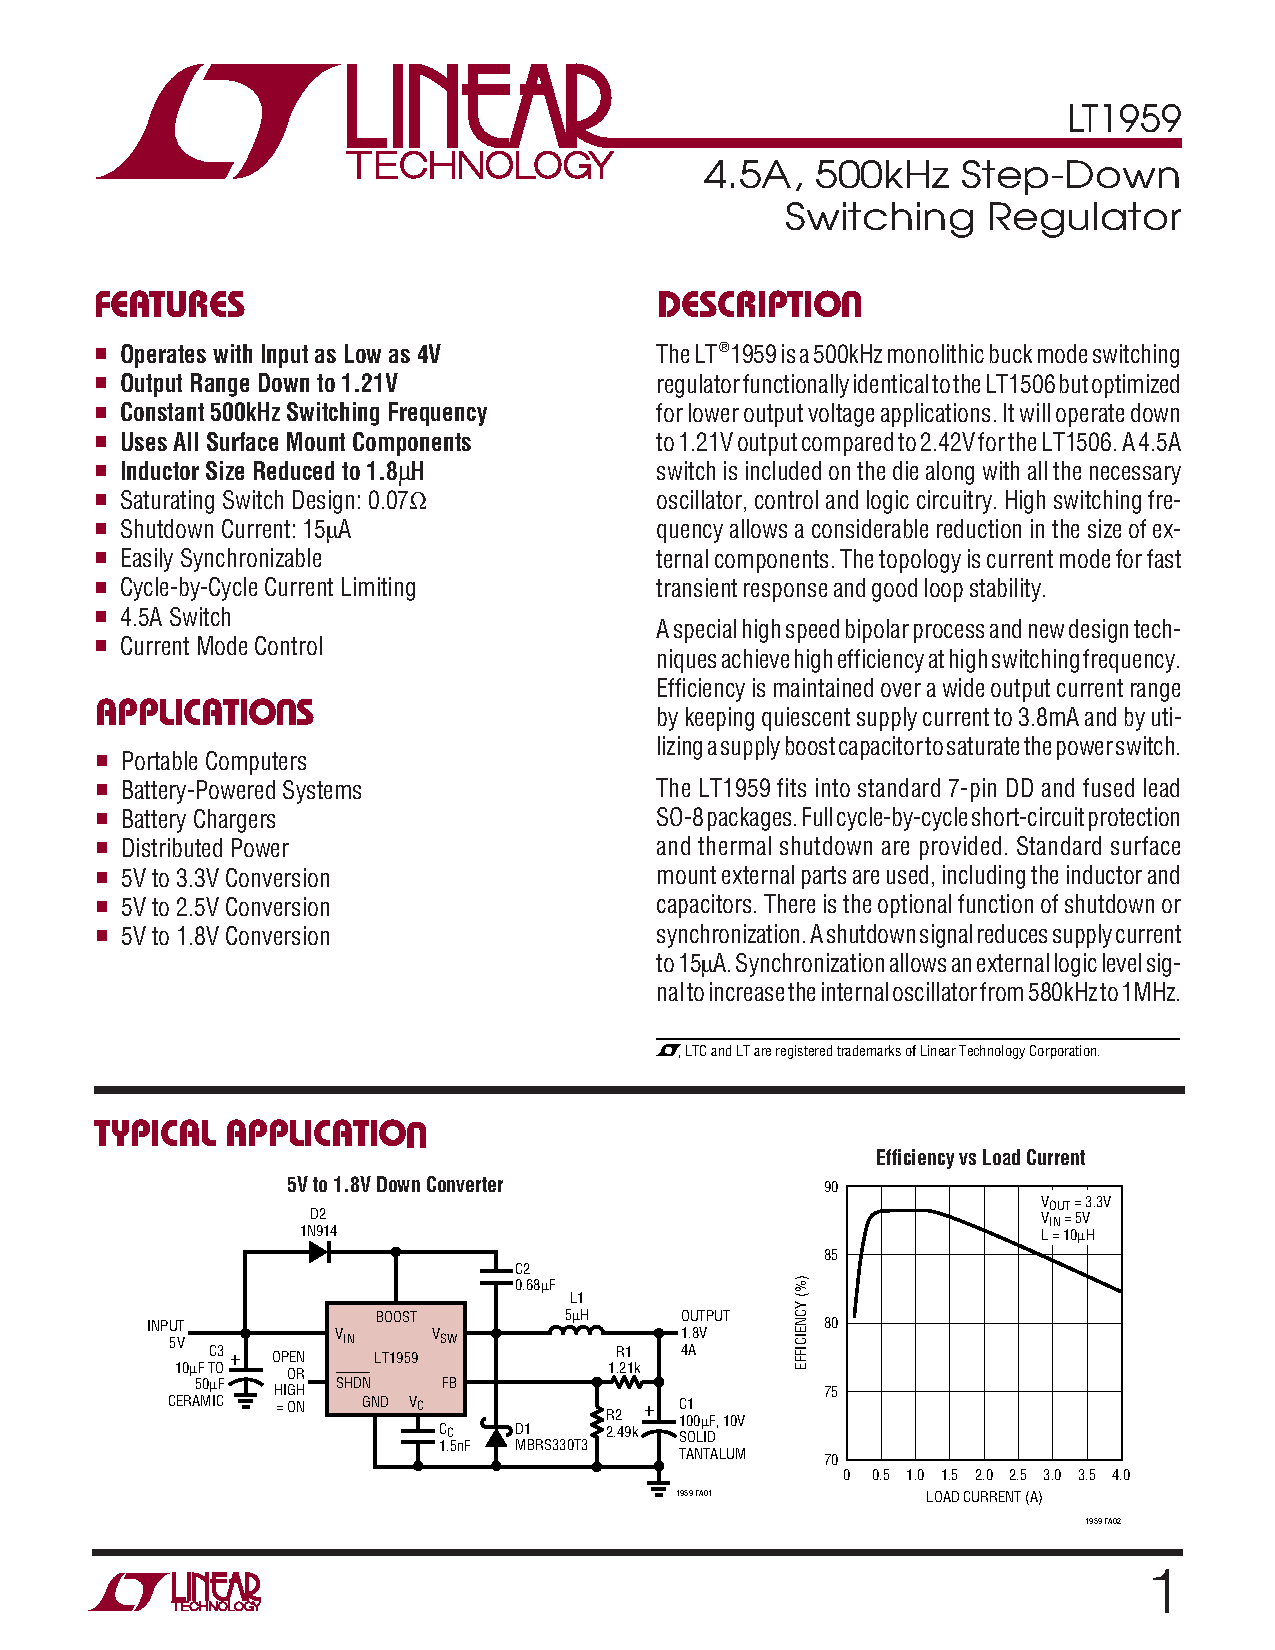
\includepdf[pages=1-4]{TD_Buck/fig/LT1959.pdf}
\includepdf[pages=6-7]{TD_Buck/fig/LT1959.pdf}